\documentclass{article}
\usepackage[T1]{fontenc}
\usepackage{lmodern}
\usepackage{graphicx}
\usepackage{amsmath,amssymb}
\usepackage[a4paper,margin=2cm]{geometry}
\usepackage[absolute,overlay]{textpos}
\setlength{\TPHorizModule}{1mm}
\setlength{\TPVertModule}{1mm}
\usepackage[indonesian]{babel}
\usepackage{hyperref}
\setlength{\emergencystretch}{2em}
% unit: Halaman 43

\begin{document}

% === Halaman 43 (python/native) ===

Dua Aplikasi Utama Enkripsi

• Enkripsi dokumen di dalam 

storage (encryption at rest)

43

• Enkripsi pesan yang dikirim 

(encryption on motion)

Sumber: https://www.scienceabc.com/innovation/how-whatsapp-app-

message-end-to-end-encryption-works-msgs-security-method-key.html

% deskripsi: gambar native xref 191
\noindent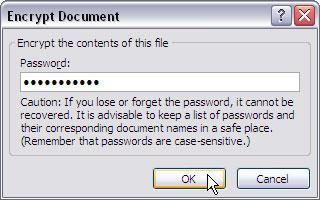
\includegraphics[width=0.85\textwidth]{../../images/python/page_043_img_01.jpeg}

% deskripsi: gambar native xref 192
\noindent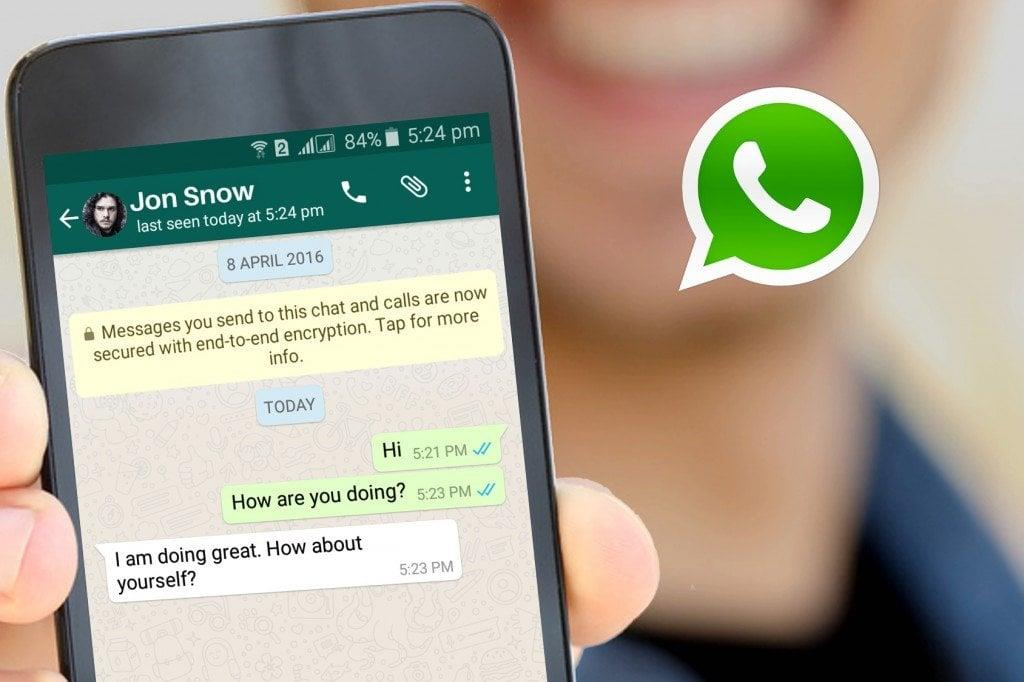
\includegraphics[width=0.85\textwidth]{../../images/python/page_043_img_02.jpeg}

\end{document}
